\chapter{Projeto - Parte 3}\label{ch:projeto-parte3}

TODO: Nesta fase do projeto, o objetivo foi criar, em \textit{python}

\section{Raciocínio Automático}\label{sec:raciocinio-automatico}

O raciocínio automático é uma área da inteligência artificial que se dedica a desenvolver algoritmos capazes de inferir conclusões a partir de um conjunto de premissas.
Pode ser visto como um processo computacional, onde se parte de uma representação de conhecimento de um determinado problema e se chega a conclusões, com base em regras de inferência (i.e., processo de manipulação de representações simbólicas para deduzir novas informações baseadas em conhecimento do domínio).

Associado ao processo de raciocínio automático, estão dois tipos de atividades principais:

\begin{itemize}
    \item \textbf{Exploração}: A exploração das opções possíveis, e que requer antecipação e previsão das suas consequências (raciocínio prospetivo) (e.g., num determinado momento, quantas jogadas possíveis existem num jogo de xadrez para que o jogador possa ganhar o jogo);
    \item \textbf{Avaliação}: A avaliação das opções exploradas, que requer a comparação das opções possíveis e a escolha da melhor opção.
    Associadas a escolha estão medidas de desempenho como o custo e o ganho (e.g., de todas as jogadas possíveis, qual a que maximiza a probabilidade de ganhar o jogo de xadrez).
\end{itemize}

De forma a resolver um determinado problema, através do raciocínio automático, é necessário representar o conhecimento do seu domínio através de representações simbólicas internas ao sistema - modelo do problema - com a informação necessária para a resolução do mesmo.
Estas representações servem de base à simulação para exploração e avaliação de opções possíveis, e são obtidas através de processos de codificação (i.e., da informação concreta do problema em estruturas simbólicas internas) e de descodificação (i.e., processo inverso).
A imagem~\ref{fig:representacao-problema} ilustra um exemplo de codificação e descodificação de um problema.

\begin{figure}[H]
    \begin{center}
        \resizebox{100mm}{!}{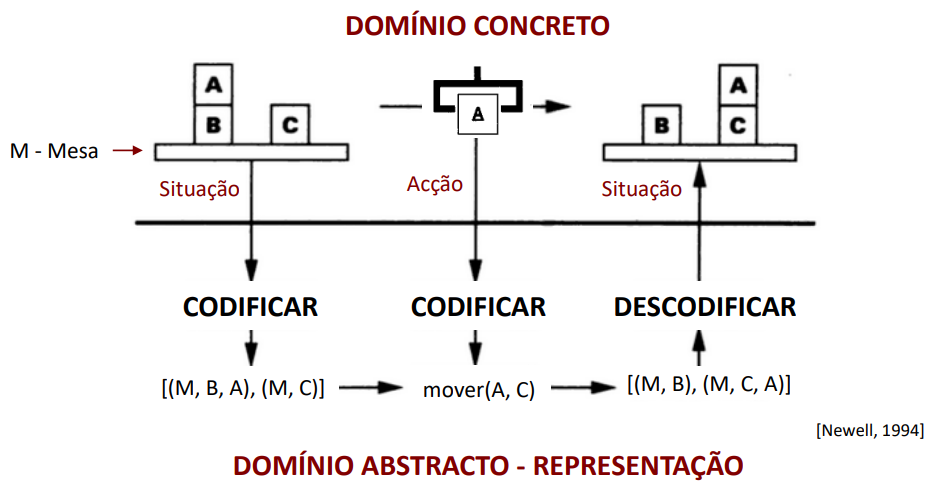
\includegraphics{../figures/representacao-problema}}
    \end{center}
    \caption{Representação de um problema.
    Retirado de~\cite{isel:iasa:slides:racicionio-automatico}, slide 8.}
    \label{fig:representacao-problema}
\end{figure}

\subsection{Modelação de um Problema}\label{subsec:modelacao-problema}

O modelo de um problema é uma representação simbólica interna ao sistema, que contém a informação necessária para a resolução do problema.
O mecanismo de raciocínio automático é responsável por manipular esta representação, de forma a inferir conclusões e a resolver o problema. Esta representação tem como base os seguintes conceitos:

\begin{itemize}
    \item \textbf{Estado}: Representação única e simbólica de um conjunto de informações concretas que caracterizam um estado da modelação de um problema. No âmbito do raciocínio automático, os estados abstraem os aspetos (configurações) estruturais que caracterizam o problema. Ao conjunto de estados possíveis de um problema e às transições entre eles, dá-se o nome de espaço de estados;
    \item \textbf{Operadores}: Representação de uma ação geradora de uma transição de um estado para outro.
    No âmbito do raciocínio automático, os operadores abstraem as transformações (dinâmicas) que ocorrem.
    Associado a um operador estão duas funções: uma que gera o estado sucessor a partir de um dado estado e outra que define o custo associado a essa transição, e que pode depender ou não do estado atual e do estado sucessor;
    \item \textbf{Transição}: Em contraste com o operador, a transição é a ação efetiva da passagem de um estado para outro (geram o estado sucessor), que ocorre quando um operador é aplicado sobre as representações internas dos estados.
    \item \textbf{Problema}: Dá suporte ao raciocínio automático, modelando um problema ao qual está inerente uma finalidade;
    Associado a um problema está o estado inicial, um conjunto de operadores e uma função predicado~\cite{stanford:fp:function-predicates} que verifica se um estado recebido é um estado objetivo ou objetivos explicítos.
    O problema considera-se resolvido quando um estado objetivo é atingido.
\end{itemize}


\section{Mecanismo de Procura}\label{sec:mecanismo-procura}

O mecanismo de procura é um dos mecanismos de raciocínio automático, que tem como objetivo encontrar uma solução para um problema de procura.

Associado a um mecanismo de procura está o conceito de árvore de procura, que é uma estrutura responsável por manter a informação gerada durante o processo de procura.
Caracteriza-se pelos seguintes conceitos:

\begin{itemize}
    \item \textbf{Nó}: Representa um estado do problema.
    Além disso, contém informação, tal como: operador (que foi aplicado para gerar o estado sucessor, e que pode não existir); antecessor (nó antecessor ao qual foi aplicado o operador para gerar este nó, e que pode não existir).
    E informação complementar para controlo do processo de procura: profundidade (do nó na árvore de procura, incremental a cada nível da árvore de procura); custo (associado ao caminho que vai do nó raiz ao nó, incremental a cada transição de um nó para o nó sucessor).
    Existe ainda o conceito de nós abertos (que ainda não foram expandidos) e nós fechados (que já foram expandidos);
    Os nós são comparáveis entre si através do seu custo;
    \item \textbf{Fronteira}: Representa os nós folhas da árvore de procura.
    Estes nós são candidatos a serem expandidos.
    A forma como é feita essa expansão dependerá da estratégia de procura utilizada (ver secção~\ref{sec:estrategias-procura});
    \item \textbf{Solução}: Representa um percurso (sequência de estados e operadores), no espaço de estados, mais concretamente, corresponde ao caminho que vai do nó raiz (estado inicial) a um dos nós objetivo (estado objetivo) encontrado.
    Podem existir várias soluções para um problema de procura, que dependem também da estratégia de procura utilizada, ou até mesmo não existir solução.
\end{itemize}

\subsection{Processo de Procura}\label{subsec:processo-procura}

O processo de procura (ver figura~\ref{fig:processo-procura}) é um processo iterativo que tem como objetivo encontrar uma solução para um problema de procura, através da exploração do espaço de estados a partir do estado inicial.
É caracterizado, de forma abstrata, pelos seguintes passos~\cite{isel:iasa:slides:proc-espaco-estados-parte-1}:

\begin{itemize}
    \item É criado um nó para representar o estado inicial;
    \item O nó é memorizado (depende da estratégia de procura utilizada);
    \item Enquanto a fronteira não estiver vazia:
    \begin{itemize}
        \item Remover um nó da fronteira;
        \item Verificar se o estado que lhe está associado é um estado objetivo.
        Se for um estado objetivo, o processo de procura termina, e é devolvida a solução que contém esse nó;
        \item O nó removido é expandido, gerando os nós sucessores;
        \item Os nós sucessores são memorizados (depende da estratégia de procura utilizada).
    \end{itemize}
    \item Se a fronteira estiver vazia, o processo de procura termina com a indicação de que não existe solução.
\end{itemize}

A expansão de um nó, mencionada no processo de procura anterior, é também um processo iterativo, que tem como objetivo gerar os nós sucessores de um nó.
É caracterizada, de forma abstrata, pelos seguintes:

\begin{itemize}
    \item Para cada operador, gerar a transição de estado do nó, que vai permitir obter o estado sucessor;
    \item Se o estado sucessor existir:
    \begin{itemize}
        \item Calcular o custo do nó sucessor (custo do nó antecessor + custo da transição para o estado sucessor);
        \item Criar o nó sucessor com o estado sucessor obtido, o operador que gerou a transição, o nó antecessor e o custo calculado anteriormente;
        \item Guardar o nó sucessor gerado numa lista.
    \end{itemize}
    \item Retornar a lista de nós sucessores gerados.
\end{itemize}

\begin{figure}[H]
    \begin{center}
        \resizebox{100mm}{!}{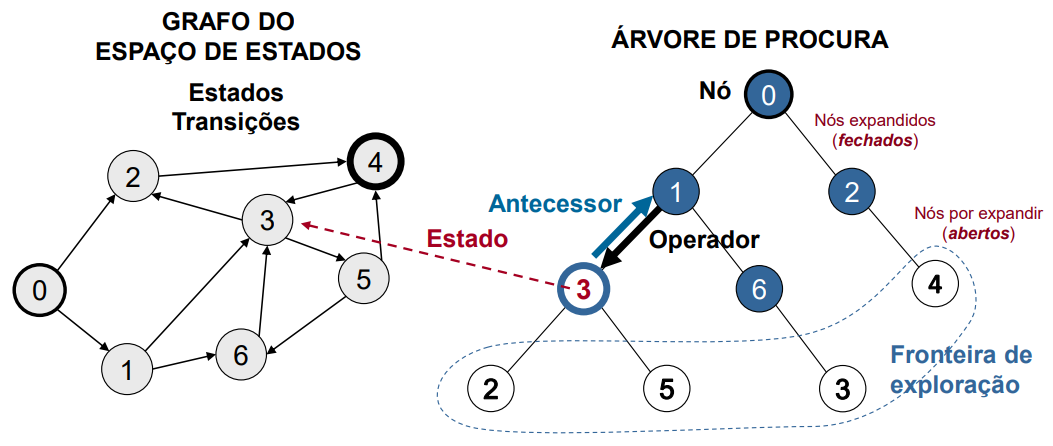
\includegraphics{../figures/processo-de-procura}}
    \end{center}
    \caption{Processo de procura.
    Retirado de~\cite{isel:iasa:slides:proc-espaco-estados-parte-1}, slide 7.}
    \label{fig:processo-procura}
\end{figure}


\section{Estratégias de Procura}\label{sec:estrategias-procura}
As estratégias de procura são responsáveis por definir a forma como a árvore de procura é explorada, ou seja, a ordem pela qual os nós são expandidos.
Existem várias estratégias de procura que se podem dividir em dois grandes grupos: estratégias de procura não informada (cega) (ver secção~\ref{subsec:procuras-nao-informadas}) e estratégias de procura informada (heurística) (ver secção~\ref{subsec:procuras-informadas}).
Além desta divisão, existe o conceito de procura em grafo (ver secção~\ref{subsec:procura-grafo}), que é uma técnica de procura que evita o aparecimento de ciclos que possam existir na árvore de procura (estados repetidos).

Alguns dos critérios de classificação das estratégias de procura são~\cite{ist:leic:resumos:procura-cega, isel:iasa:slides:proc-espaco-estados-parte-2}:

\begin{itemize}
    \item \textbf{Completa}: Se a estratégia encontra \textbf{sempre} uma solução para o problema proposto, caso exista (e caso não exista, diz que não há solução).
    \item \textbf{Ótima}: Se a estratégia encontra a solução com o menor custo possível.
    \item \textbf{Complexidade de espaço}: Espaço de memória necessário para encontrar a solução (i.e., número máximo de nós que a estratégia mantém em memória)
    \item \textbf{Complexidade de tempo}: Tempo necessário para encontrar a solução (i.e., número de operações necessárias para encontrar a solução)
    \item \textbf{Profundidade Máxima}: Corresponde à quantidade máxima de espaços entre um qualquer par de estados, ou seja, a profundidade máxima ($m$) da árvore de procura.
    \item \textbf{Fator de Ramificação}: Número máximo de sucessores de um dado nó ($b$).
    \item \textbf{Profundidade da solução}: Profundidade do nó objetivo na árvore de procura ($d$).
\end{itemize}

\subsection{Procura em Grafo}\label{subsec:procura-grafo}

Associado a uma estratégia de procura, podem estar associado o aparecimento de estados repetidos.
Tal situação leva ao desperdício de recursos computacionais (tempo e memória), uma vez que o mesmo estado é gerado e expandido várias vezes.

A solução passa por manter em memória duas listas: uma com os nós que já foram expandidos (nós fechados); e outra com os nós gerados que ainda estão por expandir (nós abertos).
No processo de memorização dos nós, associada a este processo de procura (ver secção~\ref{subsec:processo-procura}), se o nó sucessor já existir na lista de nós abertos ou fechados, é necessário verificar se o mesmo foi atingido através de um caminho mais curto (com menor custo).
Se for o caso, remover o nó anterior da respetiva lista e inserir o nó sucessor na lista de nós abertos.
Se o nó sucessor não existir em nenhuma das listas, é apenas necessário inserir o nó na lista de nós abertos.

De forma a simplificar este processamento, pode ser criada uma única lista de nós (nós explorados), onde são englobados os nós abertos e fechados. A lista deve ser indexada pelo estado do nó para eficiência de acesso, devido à elevada quantidade de nós que podem existir~\cite{isel:iasa:slides:proc-espaco-estados-parte-1}.

\subsection{Procuras Não-Informadas}\label{subsec:procuras-nao-informadas}

As procuras não-informadas (ver figura~\ref{fig:tabela-estrategias-procura-nao-informadas}), são estratégias de procura que não utilizam informação adicional para guiar o processo de procura.
Sabem apenas o que a definição do problema lhes transmite, sem qualquer tipo de pista ou heurística que permita saber se uma ação é ``mais promissora'' que outra~\cite{ist:leic:resumos:procura-cega}.
Caracterizam uma exploração \textbf{exaustiva} do espaço de estados.

\begin{figure}[H]
    \begin{center}
        \resizebox{100mm}{!}{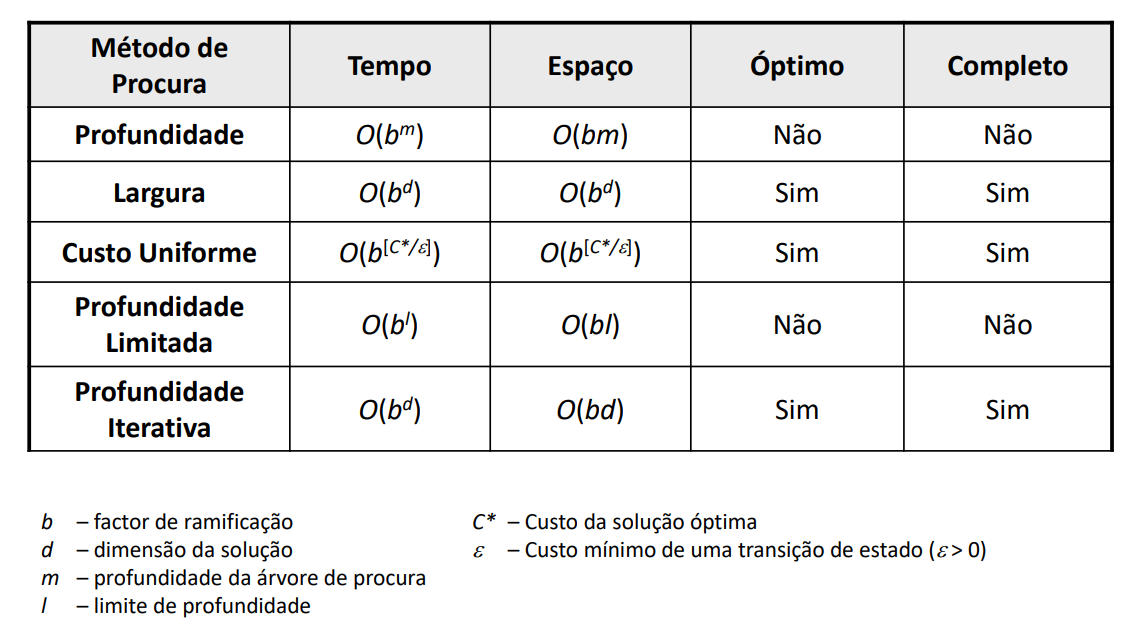
\includegraphics{../figures/tabela-estrategias-procura-nao-informadas}}
    \end{center}
    \caption{Tabela de estratégias de procura não-informadas.
    Retirado de~\cite{isel:iasa:slides:proc-espaco-estados-parte-2}, slide 12.}
    \label{fig:tabela-estrategias-procura-nao-informadas}
\end{figure}

\subsubsection{Procura em Profundidade}\label{subsubsec:procura-profundidade}

A procura em profundidade, também conhecida por \textit{Depth-First Search} (DFS), é um mecanismo de procura caracterizado por explorar um ramo da árvore de procura até ao fim antes de explorar outro ramo.
Utiliza uma fronteira de exploração do tipo \textit{LIFO} (Last In First Out), onde os nós mais recentes são inseridos no início (de modo a serem expandidos primeiro).
Este mecanismo não garante uma solução completa (visto que podem haver profundidades infinitas ou até mesmo ciclos) e muito menos ótima (já que o primeiro nó objetivo encontrado, se existir, é o que é retornado e que não é garantidamente o melhor).

A memorização dos nós, descrita no processo de procura associado (ver secção~\ref{subsec:processo-procura}) a este mecanismo, é realizada apenas através da inserção dos nós na fronteira de exploração.

O algoritmo de procura em profundidade é ilustrado na figura~\ref{fig:alg-proc-profundidade}, onde os retângulos a vermelho representam a memorização dos nós que é efetuada (ver secção~\ref{subsec:processo-procura}) no respetivo processo de procura..

\begin{figure}[H]
    \begin{center}
        \resizebox{100mm}{!}{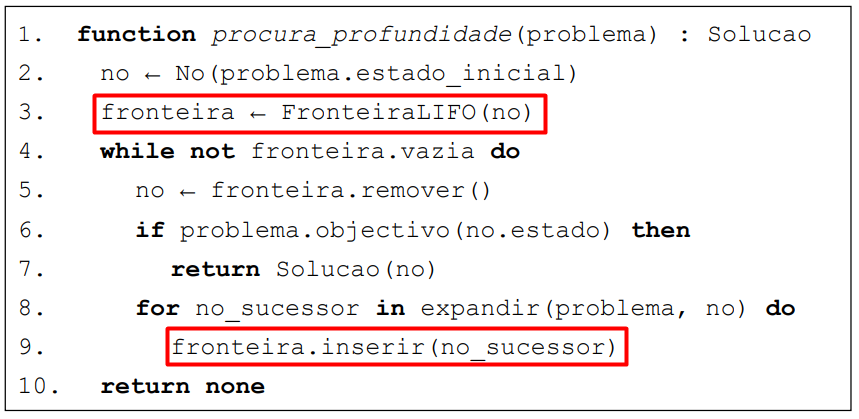
\includegraphics{../figures/alg-proc-prof}}
    \end{center}
    \caption{Algoritmo de procura em profundidade. Retirado de~\cite{isel:iasa:slides:proc-espaco-estados-parte-1}, slide 15.}
    \label{fig:alg-proc-profundidade}
\end{figure}

De notar que, a ordem de geração dos nós sucessores depende da ordem dos operadores aplicados~\cite{isel:iasa:slides:proc-espaco-estados-parte-1} e que a complexidade espacial deste algoritmo é de $O(bm)$ se for implementado de forma recursiva, e de $O(m)$ se for implementado de forma iterativa.

\paragraph{Procura em Profundidade Limitada}\label{par:procura-profundidade-limitada}

A procura em profundidade limitada, é uma variação da procura em profundidade, onde é definido um limite de profundidade, $l$, para a exploração da árvore de procura.
Com esta procura introduz-se um novo possível estado, o estado de fracasso, ou seja, se a profundidade máxima for atingida e não existir um nó objetivo, a procura termina sem solução.

Não é completa e garantidamente ótima, visto que a solução pode estar a uma profundidade maior que $l$, e que apesar de esta estratégia resolver o problema de profundidades infinitas, não resolve o problema da existência de ciclos.

O algoritmo de procura em profundidade limitada é ilustrado na figura~\ref{fig:alg-proc-prof-limitada}, onde os retângulos a vermelho representam a memorização dos nós que é efetuada (ver secção~\ref{subsec:processo-procura}) no respetivo processo de procura..

\begin{figure}[H]
    \begin{center}
        \resizebox{100mm}{!}{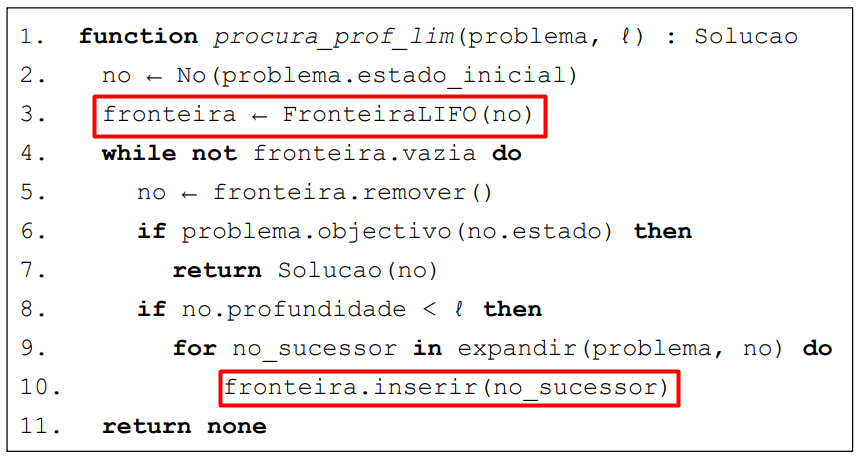
\includegraphics{../figures/alg-proc-prof-limitada}}
    \end{center}
    \caption{Algoritmo de procura em profundidade limitada. Retirado de~\cite{isel:iasa:slides:proc-espaco-estados-parte-1}, slide 17.}
    \label{fig:alg-proc-prof-limitada}
\end{figure}

\paragraph{Procura em Profundidade Iterativa}\label{par:procura-profundidade-iterativa}

A procura em profundidade iterativa, é uma variação da procura em profundidade limitada, onde é realizada uma procura em profundidade com um limite de profundidade, $l$.
Caso não seja encontrada uma solução, é realizada uma nova procura em profundidade com um limite de profundidade superior ao que foi utilizado anteriormente, e assim sucessivamente até que a solução seja encontrada.

Combina vantagens da procura em profundidade e da procura em largura, visto que a procura em profundidade é mais eficiente em termos de memória e a procura em largura é mais eficiente em termos de tempo.

É completa, caso a profundidade seja finita, e ótima, caso o custo de cada ação seja maior que zero~\cite{ist:leic:resumos:procura-cega}.

\subsubsection{Procura em Largura}\label{subsubsec:procura-largura}

A procura em largura, também conhecida por \textit{Breadth-First Search} (BFS), é um mecanismo de procura em grafo (ver secção~\ref{subsec:procura-grafo}) caracterizado por explorar todos os nós de um nível da árvore de procura antes de explorar os nós do nível seguinte. Utiliza uma fronteira de exploração do tipo \textit{FIFO} (First In First Out). Neste tipo de fronteira, os nós mais recentes são inseridos no fim (de modo a serem expandidos por último).

Este mecanismo garante uma solução completa, se o fator de ramificação ($b$) for finito, e ótima, se o custo do caminho não diminuir ao aumentar a profundidade da árvore de procura~\cite{ist:leic:resumos:procura-cega}.

O teste do nó objetivo deve ser realizado assim que o nó é gerado, para evitar processamento desnecessário (ver figura~\ref{fig:alg-proc-largura-teste}).,
já que todos os nós que existem a uma profundidade menor (com menor custo) já foram explorados e não passaram no teste.
Tal permite obter descer a complexidade temporal e espacial de $O(b^d+1)$ para $O(b^d)$, visto que um nível da árvore de procura não é explorado a mais, nem são gerados nós desnecessários nesse nível~\cite{ist:leic:resumos:procura-cega}.

\begin{figure}[H]
    \begin{center}
        \resizebox{100mm}{!}{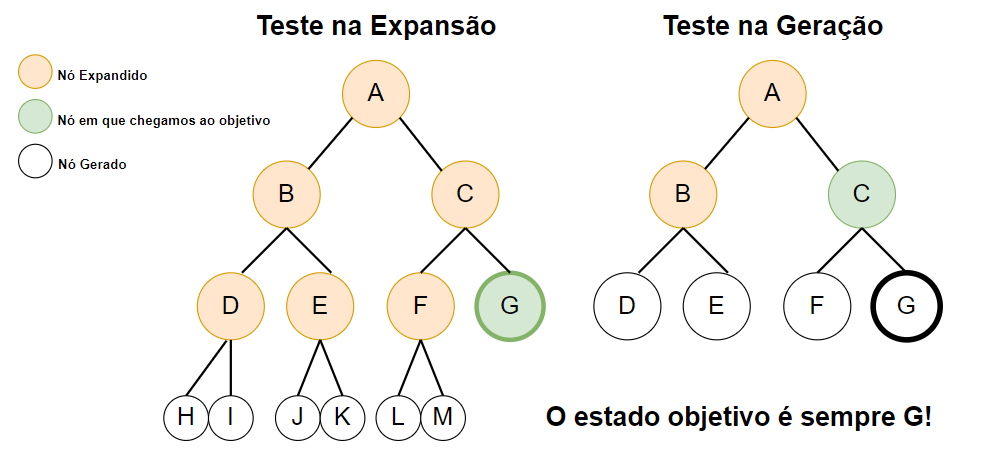
\includegraphics{../figures/alg-proc-largura-teste}}
    \end{center}
    \caption{Comparação entre o teste do nó objetivo antes e depois da expansão dos nós sucessores.
    Retirado de~\cite{ist:leic:resumos:procura-cega}.}
    \label{fig:alg-proc-largura-teste}
\end{figure}

O algoritmo de procura em largura é ilustrado na figura~\ref{fig:alg-proc-largura}, onde os retângulos a vermelho representam a memorização dos nós que é efetuada (ver secção~\ref{subsec:processo-procura}) no respetivo processo de procura. no respetivo processo de procura.

\begin{figure}[H]
    \begin{center}
        \resizebox{100mm}{!}{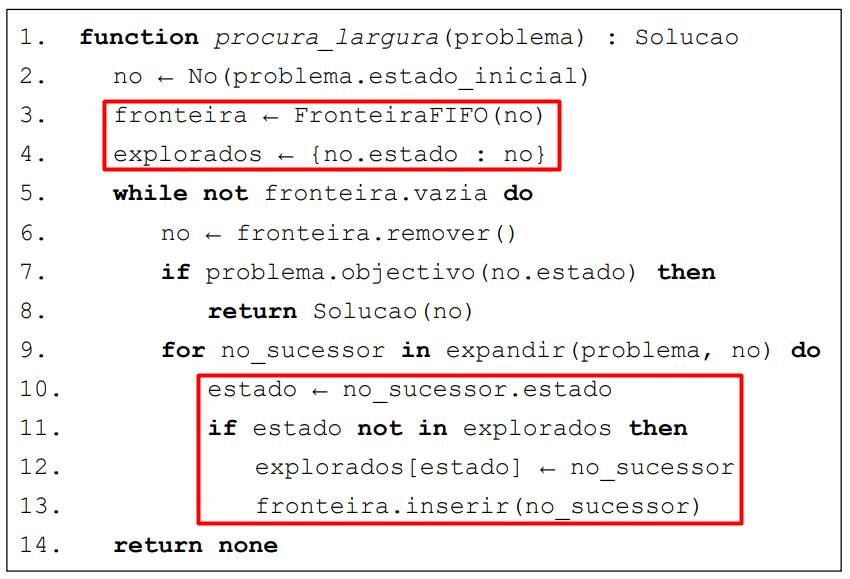
\includegraphics{../figures/alg-proc-largura}}
    \end{center}
    \caption{Algoritmo de procura em largura. Retirado de~\cite{isel:iasa:slides:proc-espaco-estados-parte-1}, slide 28.}
    \label{fig:alg-proc-largura}
\end{figure}

\subsubsection{Procura de Custo Uniforme}\label{subsubsec:procura-custo-uniforme}

A procura de custo uniforme, corresponde a um caso particular da procura por melhor primeiro (ver secção~\ref{subsubsec:procura-melhor-primeiro}), onde a função de avaliação, $f(n)$, é igual ao custo do caminho percorrido desde o estado inicial até ao nó, ou seja, $f(n) = g(n)$. Portanto, o avaliador associado a esta procura é exclusivamente a função de custo, $g(n)$.

Como a procura de custo uniforme é também uma procura por grafo (ver secção~\ref{subsec:procura-grafo}), a memorização dos nós só é realizada se os nós sucessores não estiverem na lista de nós explorados ou se o custo do nó for menor que o custo do nó explorado (ver figura~\ref{fig:alg-proc-melh-prim}).

\subsection{Procuras Informadas}\label{subsec:procuras-informadas}

As procuras informadas são estratégias de procura que utilizam informação adicional para guiar o processo de procura.
Caracterizam uma exploração \textbf{seletiva} do espaço de estados.

Este tipo de procuras, baseiam-se, de uma forma geral, na estratégia de procura de melhor primeiro (ver secção~\ref{subsubsec:procura-melhor-primeiro}).
Esta estratégia, recorre a uma função de avaliação, $f(n)$, para escolher a ordem de expansão dos nós. É o avalidor que determina o valor de $f(n)$ de um determinado nó, e que vai depender da estratégia de procura utilizada.

A função de avaliação, $f(n)$, é modelada como uma estimativa do custo entre um nó $n$, e o objetivo.
A figura~\ref{fig:proc-informada} ilustra a função de avaliação de um procura informada.
Poderá ser constituída por alguns dos seguintes componentes, através da transformação destes (soma/composição/supressão, etc..)~\cite{ist:leic:resumos:procura-informada}:

\begin{itemize}
    \item $g(n)$, o custo do caminho percorrido desde o estado inicial até ao nó $n$;
    \item $h(n)$, a estimativa do custo do melhor caminho desde o nó $n$ até ao nó objetivo,
    e que corresponde ao conceito de função heurística.
    Num nó objetivo, $h(n)$ é igual a zero;
    \item $h^*(n)$, o custo real do melhor caminho desde o nó $n$ até ao nó objetivo, isto é, a estimativa exata.
\end{itemize}

\begin{figure}[H]
    \begin{center}
        \resizebox{100mm}{!}{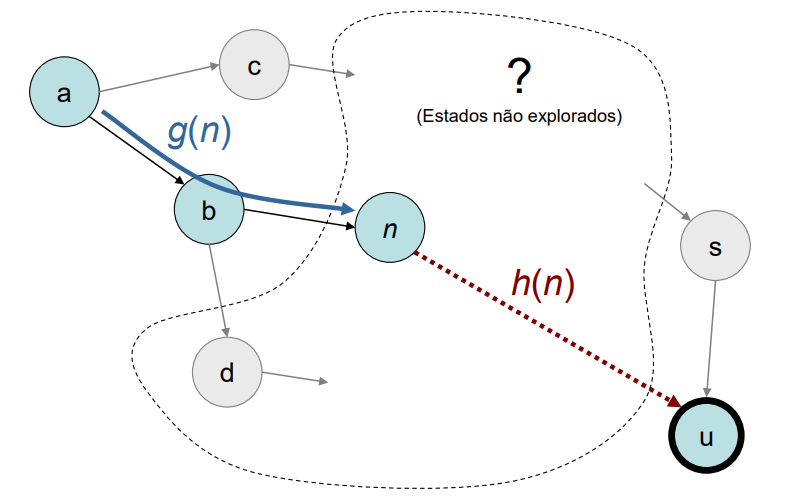
\includegraphics{../figures/proc-informada}}
    \end{center}
    \caption{Ilustração dos componentes da função de avaliação de um procura informada. Retirado de~\cite{isel:iasa:slides:proc-espaco-estados-parte-3}, slide 5.}
    \label{fig:proc-informada}
\end{figure}

Uma heurística é algo que fornece informação para resolver algo de forma expedita.
Caracterizam-se por serem estimativas rápidas e por isso não são garantidamente ótimas, não produzem indicações robustas que garantidamente levam a boas soluções, no entanto, são boas indicações e ajudam a orientar a procura.
Uma analogia seria, por exemplo, um detetor de metais, que apita cada vez mais alto à medida que se aproxima de um objeto metálico, mas não indicando, portanto, a sua localização exata~\cite{ist:leic:resumos:procura-informada}.

\subsubsection{Procura Melhor-Primeiro}\label{subsubsec:procura-melhor-primeiro}

A procura de melhor primeiro, também conhecida por \textit{Best-First Search} (BFS), é um mecanismo de procura por grafo caracterizado por expandir o nó que tem o menor valor de uma função de avaliação, $f(n)$, que é uma estimativa do custo do caminho mais curto desde o nó até ao nó objetivo.

A função de avaliação, $f(n)$, pode representar a prioridade de um nó, e é calculada através da soma de duas funções: $g(n)$, que representa o custo do caminho percorrido desde o estado inicial até ao nó $n$; e $h(n)$, que representa a estimativa do custo do melhor caminho desde o nó $n$ até ao nó objetivo.

Utiliza uma fronteira por prioridade, que internamente usa uma \textit{min priority queue}, onde os nós são ordenados de acordo com o valor da função de avaliação, $f(n)$, de forma crescente.
Desta forma, o nó com menor valor de $f(n)$ é o primeiro a ser expandido.

A procura de melhor primeiro é garantidamente completa e ótima, se a função de avaliação, $f(n)$, for admissível, ou seja, se a função heurística, $h(n)$, for menor ou igual ao custo real, $h^*(n)$, do melhor caminho desde o nó $n$ até ao nó objetivo~\cite{ist:leic:resumos:procura-cega}.

O algoritmo de procura de melhor primeiro é ilustrado na figura~\ref{fig:alg-proc-melh-prim}, onde os retângulos a vermelho representam a memorização dos nós que é efetuada (ver secção~\ref{subsec:processo-procura}) no respetivo processo de procura..

\begin{figure}[H]
    \begin{center}
        \resizebox{100mm}{!}{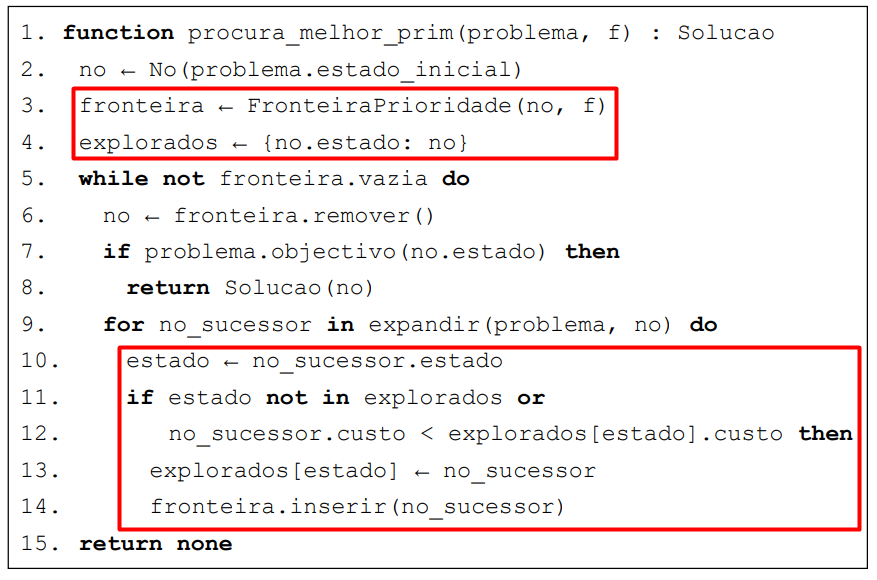
\includegraphics{../figures/alg-proc-melh-prim}}
    \end{center}
    \caption{Algoritmo de procura de melhor primeiro. Retirado de~\cite{isel:iasa:slides:proc-espaco-estados-parte-2}, slide 4.}
    \label{fig:alg-proc-melh-prim}
\end{figure}

\subsubsection{Procura Sôfrega}\label{subsubsec:procura-sofrega}

A procura sôfrega, também conhecida por procura gananciosa (\textit{Greedy Search}), é um mecanismo de procura por melhor primeiro, caracterizado por expandir o nó que tem o menor valor de uma função de avaliação, $f(n)$.
O avaliador, associado a esta procura e que determina a prioridade do nó, é exclusivamente a função heurística, $h(n)$, que representa a estimativa do custo do melhor caminho desde o nó $n$ até ao nó objetivo.

Esta estratégia tenta minimizar a estimativa de custo para atingir o objetivo não tendo em conta o percurso já explorado (só olha para a frente). Desta forma produz soluções subótimas, porque a função de heurística pode não ser admissível, ou seja, $h(n)$ pode ser maior que o custo real, $h^*(n)$.

\subsubsection{Procura A*}\label{subsubsec:procura-a-estrela}

A procura A*, é um mecanismo de procura por melhor primeiro, caracterizado por expandir o nó que tem o menor valor de uma função de avaliação, $f(n)$.

O avaliador, associado a esta procura e que determina a prioridade do nó, é a soma de duas funções: $g(n)$, que representa o custo do caminho percorrido desde o estado inicial até ao nó $n$; e $h(n)$, que representa a estimativa do custo do melhor caminho desde o nó $n$ até ao nó objetivo ($f(n) = g(n) + h(n)$).

A procura A* é garantidamente ótima, se a função de avaliação, $f(n)$, for admissível, ou seja, se $h(n)$ <= $h^*(n)$.
Isto numa procura em árvore, porque numa procura em grafo, como não são adicionados à fronteira estados por onde já passámos, podemos eventualmente perder o caminho mais curto até ao objetivo.
Este ponto, introduz um novo conceito de heurística, a heurística consistente.
Uma heurística é consistente se, para cada nó $n$ e cada sucessor $n'$ de $n$ gerado por qualquer ação $a$, o custo estimado de alcançar o objetivo a partir de $n$ é no máximo o custo de chegar a $n'$ mais o custo estimado de alcançar o objetivo a partir de $n'$.
Mais concretamente se, $h(n) <= c(n, a, n') + h(n')$, onde $c(n, a, n')$ corresponde ao custo associado a realizar a ação $n$ para $n'$~\cite{ist:leic:resumos:procura-informada}.
Esta desigualdade triangular está representada, de forma visual, na figura~\ref{fig:heur-consistente}.

\begin{figure}[H]
    \begin{center}
        \resizebox{100mm}{!}{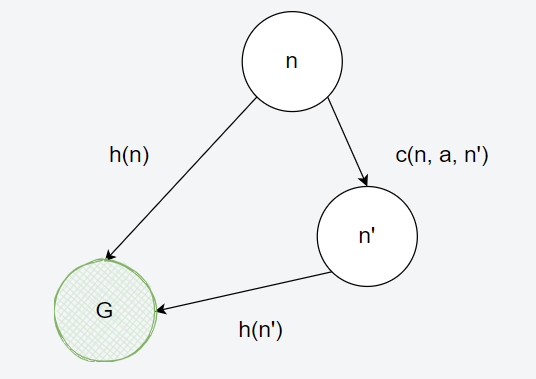
\includegraphics{../figures/heur-consistente}}
    \end{center}
    \caption{Desigualdade triangular para uma heurística consistente.
    Retirado de~\cite{ist:leic:resumos:procura-informada}.}
    \label{fig:heur-consistente}
\end{figure}

Portanto, uma heuristica admissível pode não ser uma heurística consistente, visto que o seu valor pode variar de forma não linear ao longo do processo de procura, e por isso, não respeitar a desigualdade triangular mencionada anteriormente.
E por isso, não há garantia de que um nó mais recente seja melhor que nós anteriores, ou seja, que esse nó esteja necessariamente no caminho ótimo.
Desta forma, é necessário manter os nós anteriormente explorados para comparação~\cite{isel:iasa:slides:proc-espaco-estados-parte-3}.

De notar que, uma heurística consistente é sempre admissível, visto que respeita a desigualdade triangular, no entanto, o contrário não é verdade.

Na figura~\ref{fig:comp-metodos-proc} é ilustrada a solução encontrada pela procura A* para um determinado problema, quando comparada com a procura de custo uniforme e a procura sôfrega.

\begin{figure}[H]
    \begin{center}
        \resizebox{100mm}{!}{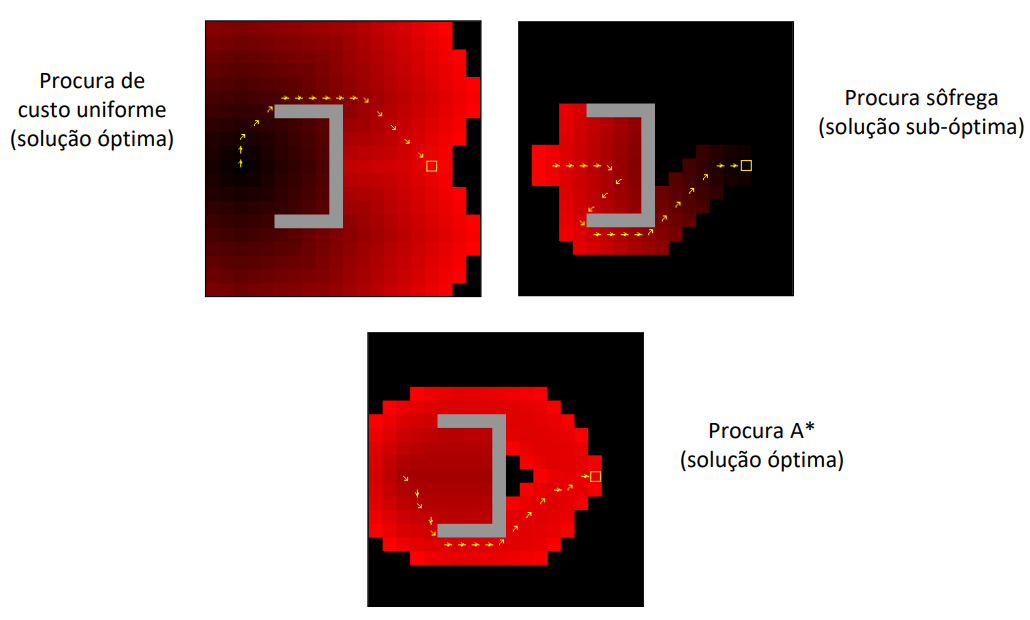
\includegraphics{../figures/comp-metodos-proc}}
    \end{center}
    \caption{Comparação entre a procura A*, a procura de custo uniforme e a procura sôfrega.
    Retirado de~\cite{isel:iasa:slides:proc-espaco-estados-parte-3}, slide 13.}
    \label{fig:comp-metodos-proc}
\end{figure}

\section{Problema de Contagem}

TODO: falar sobre como foi feita a moduleção do problema de contagem (src/contagem/)

\subsection{Escolha da Estratégia de Procura}

TODO: falar sobre a escolha da estratégia de procura e a implementação respetiva falar sobre os resultados da aplicação de cada estratégia de procura (para o problema de contagem) (src/contagem/)

\section{Estrutura do Projeto}\label{sec:estrutura-do-projeto-3}

No processo de desenvolvimento de software associado a esta fase do projeto, foi definida a seguinte estrutura em módulos e que está presente na pasta \textit{iasa\_agente/src}:

\begin{itemize}
    \item \textit{agente/contagem}: Integra a modulação que foi feita para um determinado problema de contagem, bem como o ficheiro onde lhe são aplicadas as estratégias de procura estudadas;
    \item \textit{lib/mod}: Contém classes que ajudam a modular um problema de forma abstrata (i.e., conceito de operador, estado)
    \item \textit{lib/pee}: Contém sub-módulos que permitem modular as diferentes estratégias de procura em espaço de estados estudadas:
    \begin{itemize}
        \item \textit{largura}: Contém classes que representam a estratégia de procura em largura e os seus componentes (e.g., fronteira-fifo);
        \item \textit{profundidade}: Contém classes que representam a estratégia de procura em profundidade, os seus componentes (e.g., fronteira-lifo) e variantes (e.g., profundidade-limitada, profundidade-iterativa);
        \item \textit{mec\_proc}: Contém classes que representam o mecanismo de procura e os seus componentes (e.g., no, fronteira, solução)
        \item \textit{melhor\_prim}: Contém classes que representam as estratégia de procura de melhor primeiro (e.g., procura-aa, procura-custo-unif) e os seus componentes (e.g., avaliadores)
    \end{itemize}
\end{itemize}
